%!TEX root = ../thesis-summary.tex

\section{Related Work}
\label{section:related-work}

When considering pub-sub systems, there is a set of different options that will
lay the ground for the behaviour of the whole system. We call these options,
design dimensions. Specifically, in our case, one of the biggest decisions when
designing a pub-sub system is what kind of subscription model to use. The
subscription model determines how subscribers will define which events they are
interested in. There are three major approaches covered by relevant literature
\cite{Kermarrec2013} \cite{Eugster2003} and that implementations usually
follow:

\begin{itemize}
  \item
    Topic-based subscriptions - Clients subscribe to classes of events, usually identified by keywords.\cite{Castro2002}\cite{Zhuang2001}\cite{Baldoni2007}\cite{Apolonia2018}\cite{Setty2012}
  \item
    Content-based subscriptions - Clients subscribe to events based on specific values (or ranges of values) on the properties of the events.\cite{Strom1998}\cite{Cugola2001}\cite{Carzaniga2003}\cite{Gupta2004}\cite{Bharambe2002}\cite{Voulgaris2005}
  \item
    Type-based subscriptions\cite{Eugster2000} - Bring the notion of a type scheme to a topic-based subscription model.\cite{Pietzuch2002}
\end{itemize}

The subscription models are tied to the expressiveness of the system as a
whole. Case in point, a content-based subscription model allows for a lot more
expressiveness in subscription definition. However, it makes it a lot harder to
implement a scalable way of filtering messages.

Another critical design dimension, primarily when covering P2P pub-sub systems,
is how peers choose to organise and maintain their view of the underlying
network (commonly referred to as network overlays). These overlays can usually
be divided into structured overlays, using structures as Distributed Hash
Tables (DHT) \cite{Maymounkov2002} \cite{Stoica2001} for example, and
unstructured overlays that rely on other approaches such as gossip
communication protocols \cite{Voulgaris2005a} \cite{Zheng2016}. 

The systems we will cover next have chosen different approaches for the design
dimensions described above; however, all of them have played a seminal role for
our proposed solution.

\textbf{Gryphon} \cite{Strom1998} is a content-based pub-sub system built on
top of a centralised broker hierarchy topology, successfully deployed over the
Internet for real-time sports score distribution at the Grand Slam Tennis
events, Ryder Cup, and for monitoring and statistics reporting at the Sydney
Olympics~\footnote{\url{https://www.research.ibm.com/distributedmessaging/gryphon.html}}.
Developed at IBM, Gryphon uses an interesting approach to match events with
subscriptions \cite{Aguilera1999}, relying on a distributed broker based
network to build a tree structure representing the subscription schema. 

\textbf{Siena} \cite{Carzaniga2003} is a content-based pub-sub system built on
top of a centralised broker mesh topology. Siena does not make any assumptions
on how the communication between servers and client-server works, as this is
not vital for the system to work. Instead, for server to server communication,
it provides a set of options ranging from P2P communication to a more
hierarchical structure, each with its respective advantages and shortcomings.
Still on the subject of broker based network solutions, HyperPubSub
\cite{Zupan2017} is a recent example of such an approach but focused on
bringing verifiability and other forms of decentralised validation to pub-sub
operations.

\textbf{Scribe} \cite{Castro2002} is a topic-based pub-sub system built on top
of a fully decentralised network (P2P). In order to do this, it relies on
the Pastry DHT \cite{Rowstron2001} as its overlay
structure. This allows it to leverage the robustness, self-organisation,
locality and reliability properties of Pastry to build a set of per-topic
multicast trees used to disseminate events.

\textbf{Meghdoot} \cite{Gupta2004} is a content-based pub-sub system.  It is
built on top of a P2P network, specifically CAN DHT \cite{Ratnasamy2001a}.
Meghdoot leverages the multidimensional space provided by the CAN DHT in order
to create an expressive content-based system.

\textbf{Poldercast} \cite{Setty2012} is a recent pub-sub system with a strong
focus on scalability, robustness, efficiency and fault tolerance. It follows a
topic-based model and follows a fully decentralised architecture. The key
detail about this system is that it tries to blend deterministic propagation
over a structured overlay, with probabilistic dissemination through
gossip-based unstructured overlays. In order to do this, Poldercast uses three
different overlays.\cite{Voulgaris2013}\cite{Voulgaris2005a} Similar to systems
like VCube-PS \cite{DeAraujo2017}, only nodes subscribed to a topic will
receive events published to that topic. In other words, no relay nodes are
used. It also focuses on handling churn through the use of a mixture of gossip
mechanisms, ensuring a highly resilient network.  Finally, it seeks to reduce
message duplication factor (i.e. nodes receiving the same message more than
once).

Architecturally speaking, one can see the similarities between Poldercast and
SELECT \cite{Apolonia2018}, as it too relies on a set of three different
overlays, working together to fulfil subscriptions. However, SELECT brings a
different set of properties to the table, as it maps the social connection
graph of the peers to the actual overlays operating underneath. This way, the
system can exploit both the social graph and the online activity of each social
user (each peer) to establish connections and disseminate messages accordingly
and avoid an unnecessary number of hops.

The aim of our work is also to take advantage of the network infrastructure and
technologies already in place. One of the best ways of doing so is by
leveraging what the Web platform has to offer. One cannot think of modern web
development without speaking of
\textbf{Javascript}~\footnote{\url{https://www.ecma-international.org/publications/standards/Ecma-262.htm}}.
Javascript is a lightweight, interpreted, programming language, known as the
scripting language for the web. Initially created to allow the creation of
simple interactions and animations in web pages it is now one of the main
programming languages for the web
~\footnote{\url{https://insights.stackoverflow.com/survey/2017}}, with runtimes
in browsers and servers thanks to projects such as
\textbf{NodeJS}~\footnote{\url{https://nodejs.org}}. In the application realm,
many P2P apps have leveraged these technologies. Such examples are
\textbf{browserCloud.js}\cite{Dias2018}, a solution seeking to bring cloud
computing to the Web platform, taking advantage of technologies such as
WebRTC~\footnote{\url{https://www.w3.org/TR/webrtc/}} and Javascript and
IPFS~\footnote{\url{https://ipfs.io}}, a P2P hypermedia protocol designed to
create a persistent, content-addressable network on top of the distributed web.

At the core of IPFS is what they refer to as the \textbf{Merkle
DAG}~\footnote{\url{https://github.com/ipld/specs/blob/95df205ca5fdb961ec2c2265a169989fef595db1/FOUNDATIONS.md}}.
The Merkle DAG is a graph structure used to store and represent data, where
each node can be linked to based on the hash of its content. Each node can have
links (Merkle links) to other nodes, creating a persistent, chain-like
structure that is immutable as documented in figure \ref{fig:merkle-dag}

\begin{figure}[hb!]
  \centering
  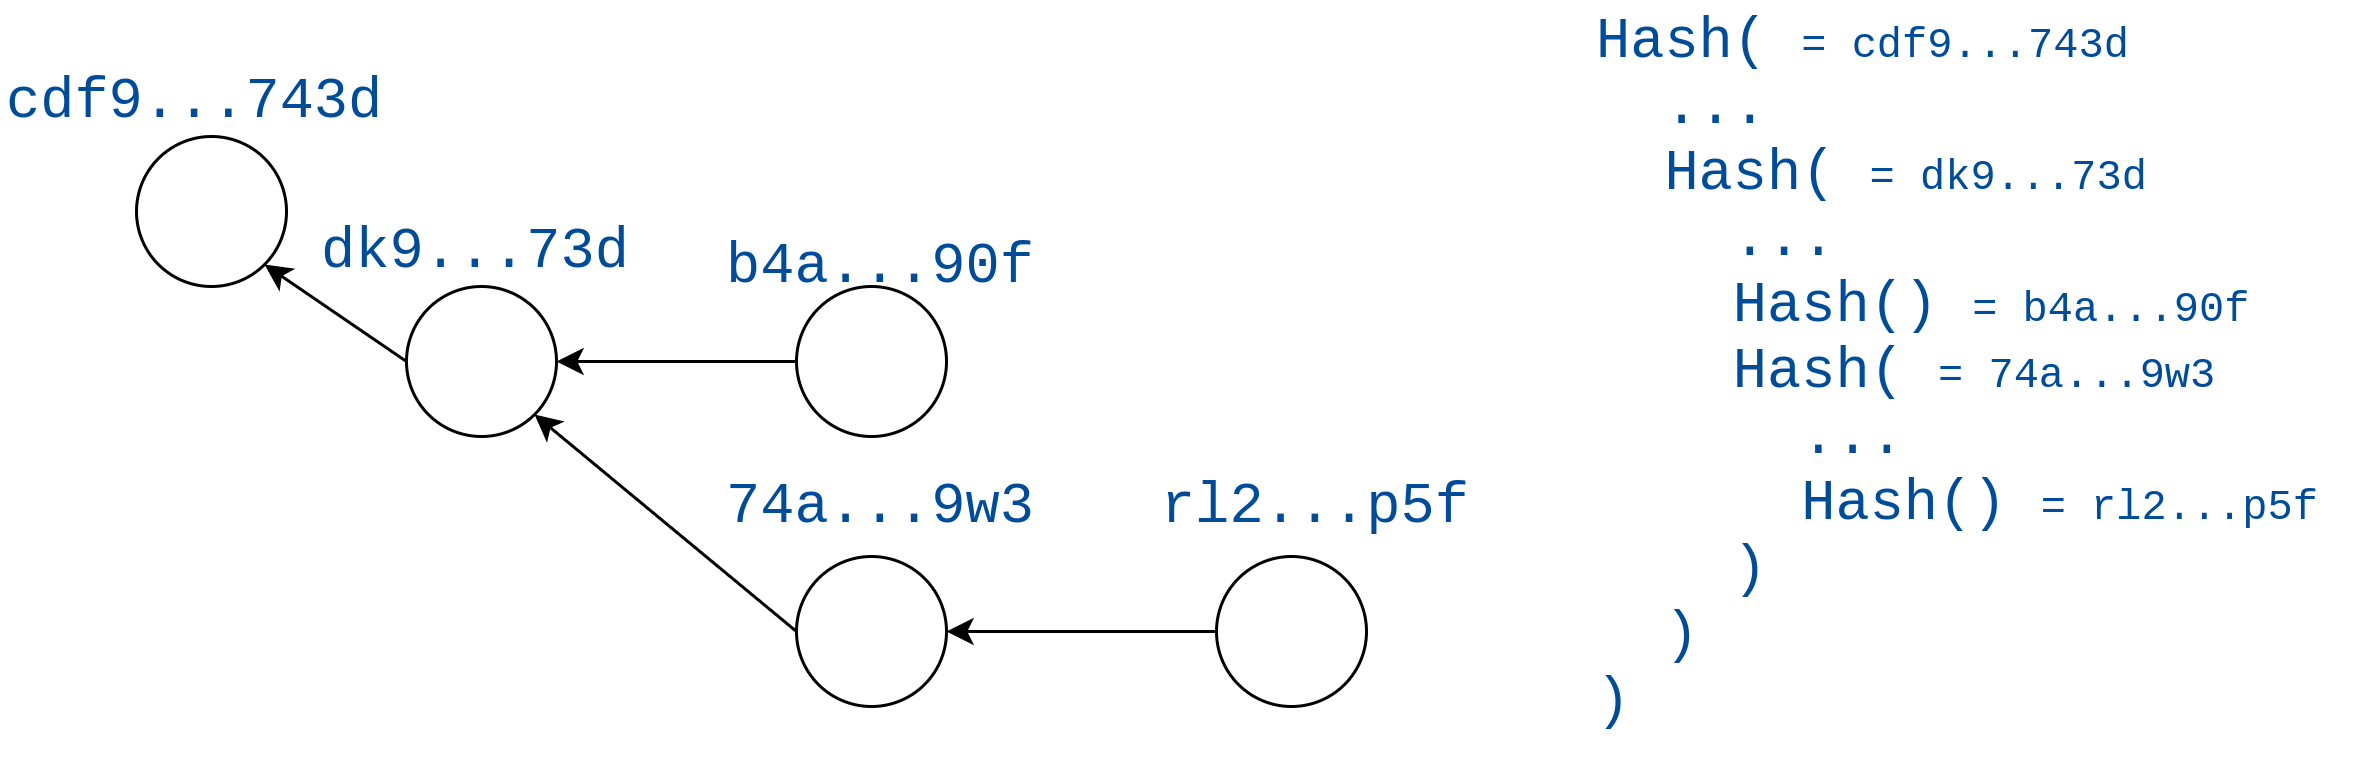
\includegraphics[width=0.3\textwidth]{img/merkle-dag.png}
  \caption{Graph visualisation of a Merkle DAG and its respective hash function dependencies}
  \label{fig:merkle-dag}
\end{figure}

Having implementations in both Go and Javascript, IPFS leverages the modularity
mantra in a fascinating way, focusing on creating standard interfaces that allow
for different pieces of the architecture to be changed and selected according
to one's needs. These small modules that constitute IPFS have recently been
brought together under the same umbrella, as
\textbf{libp2p}~\footnote{\url{https://libp2p.io}}, a set of packages that seek
to solve everyday challenges in P2P applications. Interestingly enough, a recent
addition to libp2p, and consequently IPFS, was a pub-sub module,
with a naive implementation using a simple network flooding technique, named
Floodsub. Even though libp2p was created with the initial purpose of serving as
the foundation of IPFS, it is now possible to use libp2p as a
standalone module for peer to peer apps, with the possibility to handpick the
functionalities we intend to use.
